\documentclass[10pts]{article}

%% Language and font encodings
\usepackage[english]{babel}
\usepackage[utf8x]{inputenc}
\usepackage[T1]{fontenc}
\usepackage{float}
\usepackage{listings}
\usepackage{nicefrac}
%% Sets page size and margins
\usepackage[letterpaper,top=3cm,bottom=2cm,left=3cm,right=3cm,marginparwidth=1.75cm]{geometry}

%% Useful packages
\usepackage{amsmath}
\usepackage{amsthm}
\usepackage{graphicx}
\usepackage{subcaption}
\usepackage{color}
\usepackage{xcolor}
\usepackage[colorlinks,allcolors=blue]{hyperref}
\usepackage{cleveref}
\usepackage{booktabs}
\usepackage{multirow}
\usepackage{paralist}
\usepackage{cite}
%\definecolor{codegreen}{rgb}{0,0.6,0}
%\definecolor{codegray}{rgb}{0.5,0.5,0.5}
%\definecolor{codepurple}{rgb}{0.58,0,0.82}
%\definecolor{backcolour}{rgb}{0.95,0.95,0.92}

\newif\ifdraft
\drafttrue
\ifdraft
\definecolor{ocolor}{rgb}{1,0,0.4}
\newcommand{\jwave}[1]{ {\reduwave{#1}}}
\newcommand{\jhanote}[1]{ {\textcolor{red} { ***shantenu: #1 }}}
\newcommand{\mtnote}[1]{ {\textcolor{cyan} { ***matteo: #1 }}}
\definecolor{orange}{rgb}{1,.5,0}
\definecolor{dandelion}{cmyk}{0,0.29,0.84,0}
\newcommand{\gpnote}[1]{{\textcolor{green} {***giannis: #1}}}
\newcommand{\note}[1]{ {\textcolor{magenta} { ***Note: #1 }}}
\else
\newcommand{\jwave}[1]{}
\newcommand{\jhanote}[1]{}
\newcommand{\mtnote}[1]{}
\newcommand{\gpnote}[1]{}
\newcommand{\note}[1]{}
\fi

\theoremstyle{definition}
\newtheorem{defn}{Definition}[section]

\lstdefinestyle{mystyle}{
    backgroundcolor=\color{backcolour},   
    commentstyle=\color{codegreen},
    keywordstyle=\color{magenta},
    numberstyle=\tiny\color{codegray},
    stringstyle=\color{codepurple},
    basicstyle=\footnotesize,
    breakatwhitespace=false,         
    breaklines=true,                 
    captionpos=b,                    
    keepspaces=true,                 
    numbers=left,                    
    numbersep=5pt,                  
    showspaces=false,                
    showstringspaces=false,
    showtabs=false,                  
    tabsize=2
}
 
\lstset{style=mystyle}

\title{Autonomic workload manager for executing scientific workflows on High Performance Computing resources}
\author{Ioannis Paraskevakos \\	Electrical and Computer Engineering \\
        Rutgers, The State University of New Jersey}

\begin{document}
\maketitle

\abstract{Many scientific application workflows are becoming larger and need to 
be executed multiple times with different parameters, generating a scientific 
computational campaign. Domains such as molecular dynamics, biological, and 
environmental sciences, define workflows and pipelines that are executed 
$O(1k)$ to $O(10k)$ times. In addition, based on results obtained during 
runtime the application computational requirements may change. Managing 
computational resources to reduce time to completion, maximize utilization, and 
maximize scientific insight, is becoming necessary. In this proposal, we 
present research done to understand:
    \begin{inparaenum}[(i)]
        \item scientific application time to completion characterization,
        \item scalability behavior of scientific workflows based on programming 
        models.
       \end{inparaenum}
We summarize preliminary results from our research for modeling scientific 
workflows in terms of time to completion, and propose an autonomic workload 
manager to manage workflow execution on High Performance resources. We include 
a work plan to investigate, formulate and implement the proposed workload 
manager and evaluate foreseen challenges and risks}


\section{Introduction}
\label{ch:intro}
This is the introduction of my dissertation. This document will try to show all the details of my work over the last six years.

\begin{figure}
    \centering
    \includegraphics{}
    \caption{Caption}
    \label{fig:my_label}
\end{figure}

\section{Working Definitions}
\label{definitions}
Terms such as ``workflow'', ``workload'', ``computational campaign'', and others are usually overloaded in literature and defined differently across domains. We define the terminology used in this proposal:
\begin{itemize}
    \item \textbf{Application} specifies a single or multiple tasks, and the interaction and relationship (or lack thereof) among multiple tasks. The task(s), along with their interactions and relationships represent and algorithmic solution to a science problem.
    \item \textbf{Computational Campaign} is a set of heterogeneous workflows with or without dependencies amongst them, that need to be executed.
    \item \textbf{Workflow} represents the computational instance implementing an, or part of, application with specific parameter values, number of tasks, task dependencies, and other computational aspects.
    \item \textbf{Workload} refers to a set of tasks whose dependencies have been satisfied and are ready to be concurrently executed. As such, workloads can be subsets of the tasks of a workflow.
    \item \textbf{Task} is a stand-alone process that has well defined input, output, termination criteria, and resources requirements.
    \item \textbf{Makespan} of a campaign is the time needed to execute all the workflows of the campaign, or alternatively, the maximum execution time among all paths throughout the campaign~\cite{chirkin2017execution}
    \item \textbf{Computational Objective} is a set of values selected by the user for a set of metrics which can be represented as an objective function.
    \item \textbf{Requirements} describe the minimum amount and type of resources needed to execute  each workflow of the campaign.
    \item \textbf{Constraints} are the conditions that bound the execution, including but not limited to, resource availability, capacity or costs.
    \item \textbf{Execution plan} is a sequence of actions that solves the objective function as, for example, selecting, acquiring and configuring resources, and establishing the execution order of workflows.
\end{itemize}


\section{Current Research}

TBD.

\subsection{Related Work}
\label{relatedwork}
The SelfLet framework~\cite{bindelli2008building} is an autonomic software system. 
This system provides a set of autonomic components, called SelfLets, that operate 
in order to achieve a goal. Each SelfLet provides a set of services, behaviors 
and policies. A SelfLet can be part of a network which allows it to utilize 
services from other SelfLets to achieve its goal. A SelfLet system has been used 
in a distributed sense to achieve load balanced service requests~\cite{calcavecchia2010emergence}.

The DIOS++ framework~\cite{liu2003dios} offers a rule-based autonomic management 
system for scientific applications. DIOS++ provides abstractions to create sensor 
and actuator which allow runtime monitoring and control, a distributed network to 
connect and manage the sensor/actuators and a distributed engine to execute parts 
of the application based on user defined rules.

Cloud4IoT~\cite{pizzolli2016cloud4iot} is an autonomic system which allows automatic 
deployment and configuration of data-intensive workloads on cloud and edge devices, 
and Internet-of-Things (IoT) application support. Cloud4IoT proposes an architecture 
where a Cloud is used as a central entity of computation, Edge devices are used to 
execute the initial processing steps of a data-intensive application, and IoT 
gateways are used as the gateways for sensors to connect to the system and 
transmit data.

CometCloud~\cite{diazmontes2015cometcloud} is an autonomic software system that 
enables scientific applications on a federation of resources. It has been used 
to enable simulation and data-intensive applications on heterogeneous resources, 
HPC and Cloud, that consumed million of core hours.

Pandey et al.~\cite{pandey2012autonomic} are proposing an autonomic cloud 
environment for executing multi user Electrocardiogram (ECG) data analysis 
workflows. The authors propose a three layer architecture. The ECG analysis 
software is the top layer of the architecture. The second layer contains the a 
scaling manager, a workflow engine, and a workload distribution engine. The cloud 
infrastructure and a authentication mechanism create the third layer of the 
architecture. All three layers are provided as a Service.

\gpnote{Workload management systems..........}


\subsection{Conceptual Model for Task-Parallel framework selections}
Tasks-parallel applications involve partitioning a workload into a set of 
self-contained units of work. Based on the application, these tasks can be 
independent or coupled with varying degrees of data dependencies. Scientific 
workflows exploit task parallelism for simulations as well as data analysis.

In~\cite{paraskevakos2018task}, we investigated the suitability of task-parallel 
frameworks for Molecular Dynamics trajectory data analysis. The analysis included 
Spark~\cite{zaharia2010spark}, Dask~\cite{rocklin2015dask}, and RADICAL-Pilot~\cite{merzky2019using}. 
Spark~\cite{zaharia2010spark} and Dask~\cite{rocklin2015dask} are two Big Data 
frameworks. Both provide MapReduce abstractions and are optimized for parallel 
processing of large data volumes, interactive analytics and machine learning. Their 
runtime engines can automatically partition data, generate parallel tasks, and 
execute them on a cluster. In addition, Spark offers in-memory capabilities allowing 
caching data that are read multiple times, making it suited for interactive 
analytics and iterative machine learning algorithms. Dask also provides a MapReduce 
API (Dask Bags). Furthermore, Dask’s API is more versatile, allowing custom 
workflows and parallel vector/matrix computations. RADICAL-Pilot~\cite{merzky2019using} 
allows concurrent task execution on HPC resources. The user defines a set of 
Compute-Units (CU) - the abstraction that defines a task along with its dependencies - 
which are submitted to RADICAL-Pilot. RADICAL-Pilot schedules these CUs to be 
executed under the acquired resources. It uses the existing environment of the 
resource to execute tasks and any data communication is done via an underlying 
shared filesystem.

The MD analysis algorithms investigated were selected from MDAnalysis~\cite{gowers2016mdanalysis,michaud2011mdanalysis}.
 MDAnalysis is a Python library that provides a comprehensive environment for 
 filtering, transforming and analyzing MD trajectories in all commonly used file 
 formats. It provides a common object-oriented API to trajectory data and leverages 
 existing libraries in the scientific Python software stack, such as NumPy~\cite{numpy} 
 and Scipy~\cite{scipy}. The first algorithm is embarrassingly parallel and has 
 no dependencies between tasks, while the second algorithm is a MapReduce 
 algorithm.

\begin{figure*}[t]
    \centering
    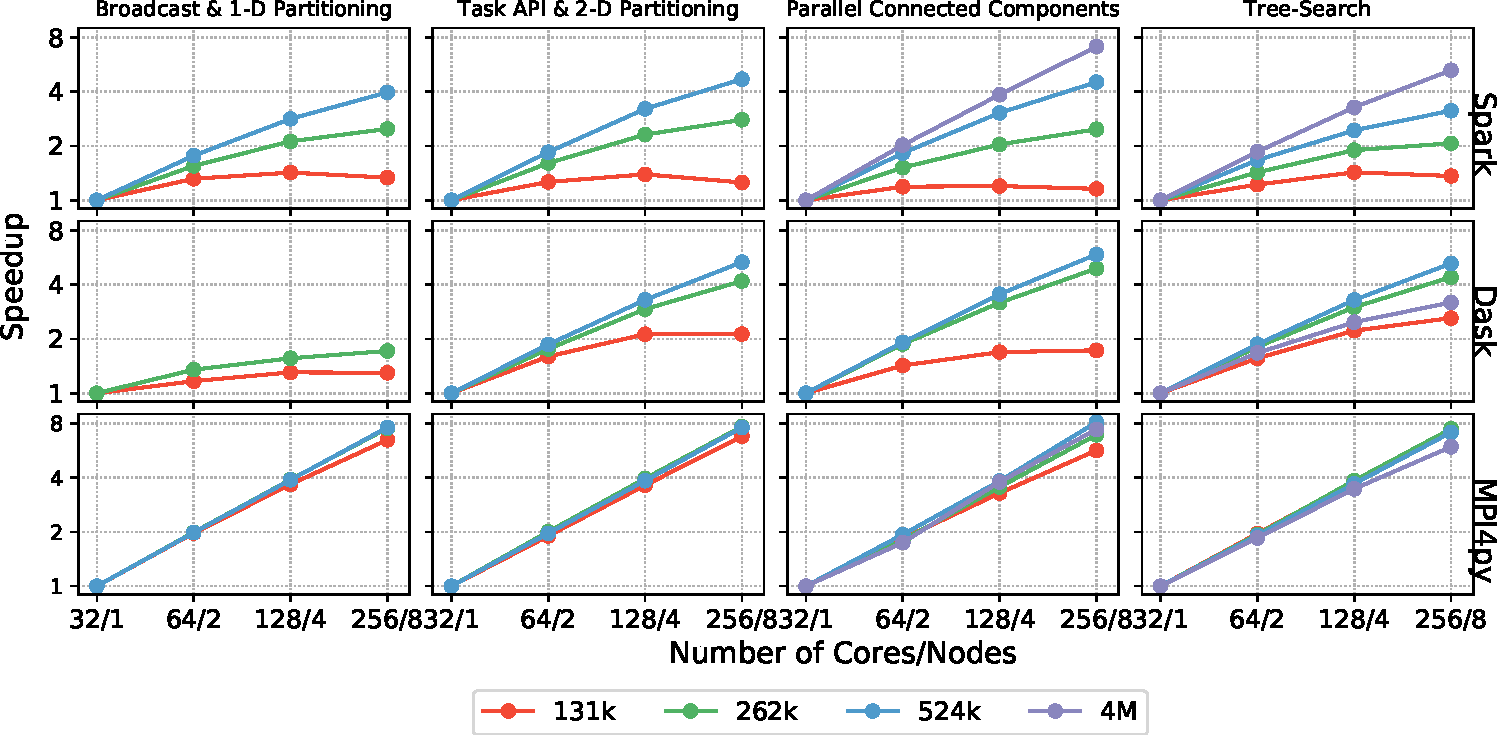
\includegraphics[width=.95\textwidth]{figures/All4approachesWith4MSpeedup.pdf}
    \caption{Selected molecular dynamics analysis MapReduce algorithm speedup for different frameworks and implementation candidates}\label{fig:leafletfinder}
\end{figure*}

The performance analysis of these algorithms implemented in all three 
frameworks provided us with information to create a conceptual model for selecting 
the better suitable framework based on algorithmic characteristics. As shown in Figure~\ref{fig:leafletfinder}, there are cases where the performance of a parallel implementation is far from ideal, while under different circumstances is as expected. Furthermore, non-ideal performance indicates that resource utilization is low. For example in Figure~\ref{fig:leafletfinder}, we see that, based on data sizem Dask provides better speedup than Spark. In these cases Dask better utilized the resources compared to Dask, while on others Spark was better.

Implementation  aspects, such as computational complexity, and shuffled data size influence 
the performance greatly. For embarrassingly parallel applications with coarse grained 
tasks the choice of the framework does not significantly influence performance. 
For fine-grained data parallelism, a data-parallel framework is more suited compared 
to a workload execution framework. In addition, the data shuffling size significantly 
impacts performance and needs to be included in a decision.

Data analysis during scientific campaigns may vary depending on the stage of the 
campaign. As a result, the ability to select the best suited framework, given 
requirements and constraints to execute it is important. This work allows us to 
create that decision making process and include it in the proposed work.

\subsection{Data Analysis Design Selection}
\gpnote{Write about publication number 2}

\section{Proposed Research}

In our research so far, we discussed a conceptual model for data analytics for 
various use cases on HPC system, and a design comparison and execution time 
model for scientific workflows. In addition, we identified a need for execution 
of  scientific workflows with minimum user intervention, independent from 
users' scientific domain. In this section, we motivate and propose an 
autonomic middleware for configuring, monitor and adapting the execution of 
scientific workflows on HPCs.

\subsection{Proposed Topic}

\label{research}
So far, we discussed an extension of the pilot abstraction to support data analytics and task based data intensive applications on HPC resources, a comparison between different task-based data oriented frameworks, and a design comparison for executing scientific workflows.
In this section, we motivate and propose a Campaign Manager (CM) to execute scientific campaigns via creating and enacting a campaign execution plan on heterogeneous and dynamic HPC resources. \mtnote{Do we need to explain how these three topics fit together?}\gpnote{I am not sure}

\subsection{Proposed Topic}
Scientific campaigns execute workflows on heterogeneous resources either with a given objective~\cite{casajus2010dirac} and/or for large periods of time~\cite{maeno2008panda}.\mtnote{I think the two are not mutually exclusive: executions of campaigns can have both a given objective and run for a large period of time.}
This objective can be translated to a computational objective function that would either minimize or maximize a metric.
Calculating the makespan of the campaign means finding the execution plan that satisfies the computational objective function.


\mtnote{Following the work we did on the separated scratch document, here a brief summary of the 'story' we agreed upon: 
\begin{enumerate}
    \item  General description of the problem space in terms of homo/heterogeneity of campaigns' workflows/resources with the help of the diagram in Figure 1, iterated to show the relevance of space heterogeneity; 
    \item initial formal definition of TTX\_w, including revised list of explicit assumptions, argument about abstraction from resource implementation, list of symbols, and first three equations (r=1, w=\{space/time homo*, space/time hetero*\}; r=n,  w=\{space/time homo*\}; r=n,  w=\{time hetero*\}); 
    \item propose to expand this initial model in the next year by: 
    \begin{enumerate}
        \item relax assumption about homogeneous resources; 
        \item add type heterogeneity of both r and w; 
        \item define m algorithmically; 
        \item if there is time, propose a quantitative definition of m.
    \end{enumerate}
\end{enumerate}}
\gpnote{moved it here}

The way workflows of a given campaign are mapped to resources can affect the makespan of the campaign. 
Figure~\ref{fig:example_makespan} shows an example of a campaign with heterogeneous workflows, and the makespan two different mappings produce.
The makespan of the campaign on the left subfigure is $20$, while on the right it is $16$.
In addition, the size of the workflows, i.e., the number of resources they require, becomes relevant and resources may be underutilized, as shown in Figure~\ref{fig:example_makespan}.

\begin{figure*}[ht!]
    \centering
    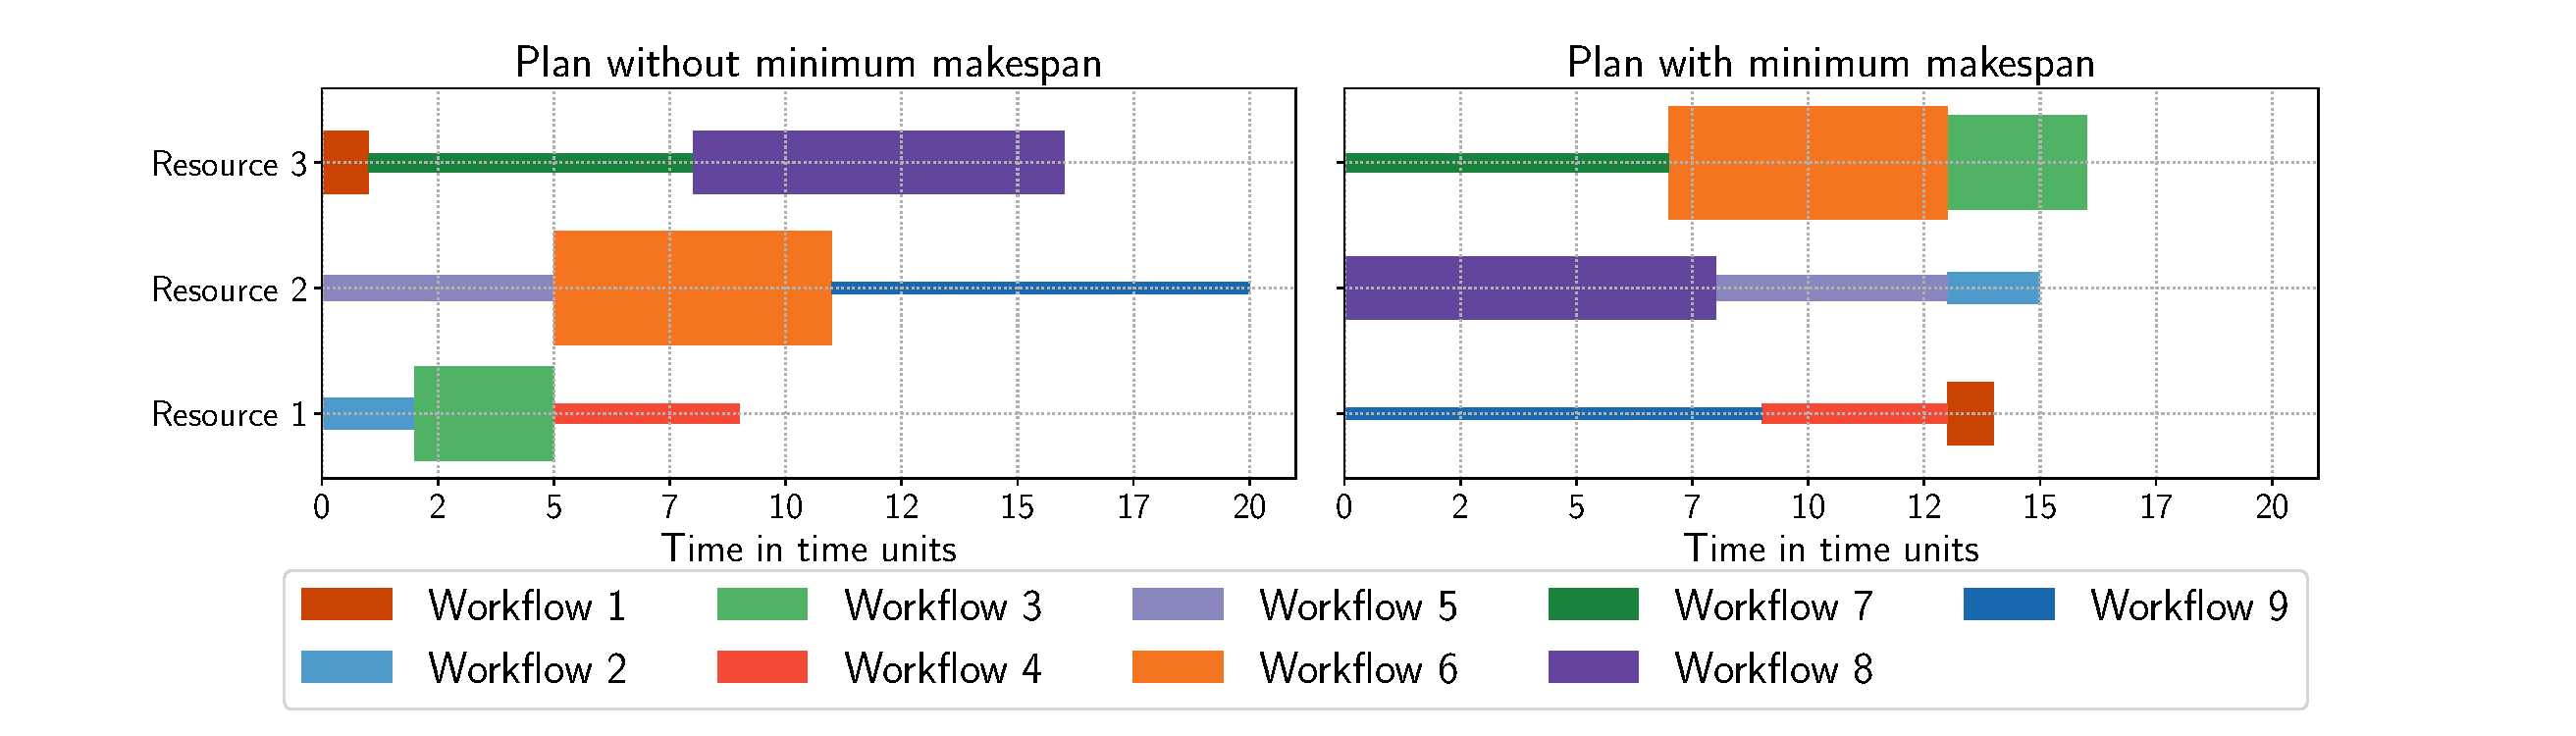
\includegraphics[width=.95\textwidth]{figures/random_vs_specific.pdf}
    \caption{Comparison of different campaign execution plans. Based on workflow mapping on resources makespan and resource utilization is different.}\label{fig:example_makespan}
\end{figure*}

We are making a set of assumptions which we do not relax during our initial analysis.
These are:
\begin{inparaenum}[(1)]
    \item a workflow is an atomic unit and cannot be decomposed;
    \item workflow resource request is sufficient to execute the workflow and the requested resources are utilized;
    \item a resource is an aggregate of computing capabilities;
    \item every workflow of a given campaign can be executed;
    \item a random resource selection is based on a uniform distribution;
    \item only one workflow can be executed on a resource at any point in time; and
    \item a workflows can be homogeneous or heterogeneous in space---maximum number of resources they need, and time---the amount of time they are executing.
\end{inparaenum}

We denote a computational campaign as $w = [w_{i}: 1 \leq i \leq W]$, where $w_{i}$ is a workflow and $W$ is the total number of workflows, $r = [ r_{j}: 1 \leq j \leq R]$ is a set of available resources, where $r_{j}$ is a resource and $R$ is the total number of available resources, and $ m(w,r) = [(w_i, r_j): 1 \leq i \leq W, r_j \in r] $ is a mapping function of workflows onto resources.
In addition, we denote as $TTX_{w_{i}}$ the execution time of a workflow, $TTX_{w}$ as the makespan of campaign $w$, and $TTX_{w}^{m}$ as the makespan of campaign $w$ for a given mapping function $ m $.
Assumption~\#3 allows to abstract the resource implementation, as workflows can be executed on different resources such as HPCs, Clouds, pilots and more. 
Lastly, we will assume homogeneous resources as it simplifies the formalization of the problem.

Assuming a single resource, i.e., $R = 1$, the workflows of the campaign will be executed sequentially, whether the workflows are homogeneous or heterogeneous.
As a result the makespan of the campaign is
\begin{equation}
   TTX_{w} = \sum_{i=1}^{W}TTX_{w_{i}} 
\end{equation}

When assuming multiple homogeneous resources, i.e., $1 < R < W$, the workflows can be executed concurrently.
Furthermore, this is semantically equivalent to executing on a single resource large enough to allow concurrent workflow execution, where each workflow executes on resource partition. 
Because of assumptions~\#4 and~\#6, executing homogeneous workflows or heterogeneous in space workflows is the same.
A random mapping of workflows onto resource will have a makespan
\begin{equation}
   TTX_{w}^{random} \geq \frac{1}{R}\sum_{i=1}^{W} TTX_{w_{i}} 
\end{equation}
When executing workflows heterogeneous in time, whether they are heterogeneous in space or not as well, on multple homogeneous resources, the makespan of the campaign for a given mapping function $ m $ is

\begin{equation}
TTX_{w}^{m} = \max_{r_{j}\in r}\Big\{\sum_{r_{i}\in m(w,r_{j})}TTX_{w_{i}}\Big\}
\label{eq:makespan}
\end{equation}

During the next year, we propose to expand the model, as it is represented in equation~\ref{eq:makespan}, by relaxing some of the initial assumptions.
First, we will relax the assumption that resources are homogeneous in terms of (1) maximum number of resources they have available; (2) type of resources, e.g., CPUs or GPGPUs; and (3) the time they are available.
Second, we will add resource type heterogeneity of workflows.
As a result, workflows will not be able to be executed on all available resources affecting the way the makespan is being calculated.
Furthermore, we propose to explore algorithmic instances of the mapping function $ m $, and if there is time, we will propose a quantitative definition of $ m $.

\mtnote{I think that we will need either equations or diagrammatic representation of the placement + makespan, ideally both. Even knowing quite well what you are trying to write, it is very difficult to follow your argumentation. There are elements of the argumentation (assuming I understand it well enough) that I might disagree with but I am going to keep those thoughts for after the proposal :)}
\gpnote{separate document moved here.}

% ----------------------------------------------------------------------------
% campaign makespan modeling
We propose to utilize and extend the Heterogeneous Earliest Finish Time (HEFT)~\cite{topcuoglu2002performance} algorithm  as an initial candidate of the mapping function $ m $\mtnote{for doing what?}\gpnote{any better?}.
HEFT is an offline scheduling algorithm which calculates the makespan of a workflow on heterogeneous resources, in terms of performance.
HEFT has been implemented as part of the planning capabilities in Pegasus~\cite{deelman2015pegasus} and ASKALON~\cite{fahringer2005askalon} amongst other algorithms.
HEFT provided better performance in terms of makespan minimization when compared to a random or round robin plan~\cite{deelman2015pegasus}.
This makes HEFT a good candidate for minimizing the makespan of a campaign.


HEFT makes two important assumptions when used to work upon workflows.
First, any task in a workflow can be executed in all available resources, and second all resources are always available.
HEFT is mainly used to derive and execution plan for workflows, i.e. the execution order and resource placement of the tasks that comprise the workflow.
Because we are interested in campaigns, our HEFT extension will provide an execution plan based on workflows as the unit it will operate.
HEFT uses a matrix to represent execution time of tasks on resources, assigning tasks to the resource that minimizes the finish time of the task, and has complexity proportional to the number of dependencies between tasks and the number of resources offered.\mtnote{Why suddenly are we writing about tasks? What is the relationship between HEFT, tasks, workflows and campaigns?}\gpnote{HEFT was created to work on workflows. I added the next paragraph to show how HEFT for campaigns might be different.}
Furthermore, there has been some initial research to extend HEFT to resources that provide CPU and GPUs~\cite{shetti2013optimization}, as well as a HEFT extension on dynamic resources~\cite{dong2007pfas}.

We identify four points of possible extensions, so that HEFT is utilized for campaigns.
These are:
\begin{inparaenum}[(i)]
    \item selecting resource that can execute a given workflow,
    \item taking into account dynamic resources, as they may become unavailable during execution,
    \item multiple workflows may be executed in a single resource concurrently, and
    \item including user specified priorities for workflows.
\end{inparaenum}
Because workflows are heterogeneous, we assume that there is at least one resource can satisfy the computational requirements of any workflow in the campaign, but not necessarily all resources.
Resources may become unavailable because the user has no allocation left, a scheduled maintenance is taking place, or due to some unscheduled downtime.
During the execution of a campaign, some workflows may have a higher priority compared to other due to user preference, or as response to an unforeseen event.
As a result, HEFT's data structure and HEFT needs to be extended to identify whether a workflow can be executed in a given resource or not, whether a resource is available or not, and user provided initial priorities.
Finally, a resource may have enough capacity so that multiple workflows can be executed concurrently.
We will investigate how HEFT can be extended to support variable resource capacity.\gpnote{It may need further extension.}

There are several alternative methods and algorithms to calculate and optimize the makespan of a workflow~\cite{lu2019review}, including queuing networks~\cite{yao2019throughput,bao2019performance}, domain specific languages~\cite{carothers2017durango,maheshwari2016workflow}, and machine learning~\cite{witt2019predictive,pumma2017runtime}.
Queuing networks will be of limited use because they require from the user to provide a queuing network equivalent to the campaign.
In the case the campaign contains only independent workflows, a single queuing system with multiple servers would be sufficient, but a campaign with complex dependencies between workflows may require expertise outside of the user domain to define the equivalent queuing network.
HEFT sorts workflows based on the number of dependencies they have in the campaign.
Furthermore, using queuing systems to derive the makespan of a campaign requires to search for possible mappings and keep the one that optimizes the makespan.
HEFT provides as an output, the plan that minimizes the makespan.
\mtnote{These two sentences are unclear, please revise.}\gpnote{any better?}

Domain specific languages approaches either require description of the resource usage of workflows~\cite{carothers2017durango}, or execute part of the campaign to obtain execution skeleton of the campaign~\cite{maheshwari2016workflow}.
When executing a campaign, workflows may require days to execute to obtain execution time information, and users rarely know the resource usage of their workflows to provide enough useful information.
In addition, the workflows of a campaign may be different and executing some of them may not provide any information about the execution of others.
HEFT also requires an initial estimation of the execution time of the workflows. We plan to utilize initial estimations provided by the users and update the values as workflows are being executed.
\mtnote{This is unconvincing: we choose to use the PST model and then we say that it requires too much effort? Remember: the argumentation here has to be `scientific', not just based on 'I want to use EnTK so this would require too much time'.}\gpnote{I removed the EnTK argument.}
Similarly, machine learning approaches would be of limited use since there is no guarantee that the workflows of a campaign is are going to be similar.
As a result, to gather enough information to build a makespan calculation model may require the execution of the campaign\mtnote{Why would this be a problem?}\gpnote{changed it}.
We want to provide an approach that only requires the user to provide as few information as possible, such as the workflows and an educated guess of their execution time\gpnote{any better?}.

% ----------------------------------------------------------------------------
% Campaign Manager definition, requirements, features and capabilities
We propose to design a campaign manager (CM) which, given a campaign, an objective, and a set of constraints, can derive an execution plan by utilizing the proposed makespan HEFT algorithm, and execute a campaign.
If necessary the CM will change the execution plan by updating workflow to resource mapping, and resource availability.
Execution planning for workflows are provided by several workflow execution systems, such as Pegasus~\cite{deelman2015pegasus}, and ASKALON~\cite{fahringer2005askalon}.
Campaign management systems, such as PanDA~\cite{maeno2008panda}, do not provide a campaign planning feature.
QCFractal~\cite{qcfractal} offers some form of planning by allowing user to specify the priority of a workflow in a campaign, but it does not plan with taking into account the makespan of the campaign.\mtnote{only these two among all the existing systems? Please refine and expand, explaining that these are just examples. Also, expand appropriately introducing the notions of planning and plan and explaining why they relate to campaign management.}\gpnote{I introduced the plan a few paragraphs before. It may still need to be expanded.}

Currently, campaign managers are making assumptions about the resources and the middleware they are utilizing, are monolithic software systems, and/or they are domain specific.
The proposed CM will support multiple use case from different domains, such as molecular dynamics and earth sciences.
As a result, it is domain agnostic.
In addition, the proposed CM prototype will be designed based on the building blocks approach~\cite{turilli2019middleware}.
As a result, the proposed CM will be agnostic of the system it interfaces to execute workflows.
This, in turn, allows the CM to make no assumptions about the resources and the middleware that is utilized for workflow execution.

Figure~\ref{fig:refarch} shows a reference architecture where the CM has three components:
\begin{inparaenum}[(1)]
\item a Planner,
\item and Enactor, and
\item a Bookkeeper. 
\end{inparaenum}
Workflow execution will be done through an existing workflow management framework (WMF) on HPC resources.
Plan updates will be based on workflows execution metrics provided by the selected WMF such as tasks execution time, overheads calculation and time to completion.
These metrics will be aggregated across workflows resulting in campaign-wide execution metrics.

\begin{figure*}[t]
    \centering
    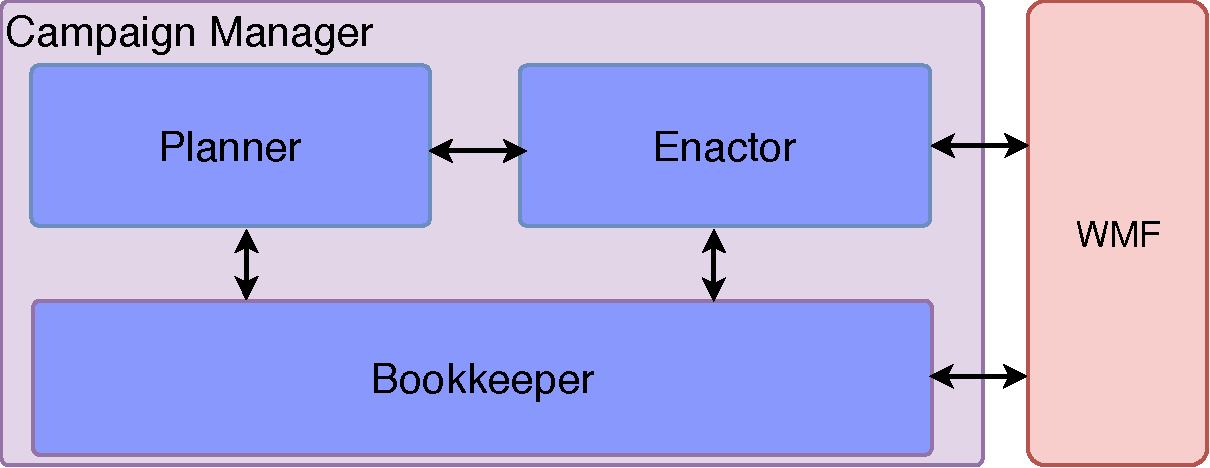
\includegraphics[width=.95\textwidth]{figures/CEM_design.pdf}
    \caption{Reference Architecture of a Campaign Manager. Basic 
    components of Campaign Manager (CM): 1) Planner, 2) Enactor and 3) Bookkeeper. 
    CM communicates decisions to RADICAL-EnTK. CM communicates with HPCs to 
    execute parts of the campaign.}\label{fig:refarch}
\end{figure*}

The Planner is responsible to derive an execution plan by calculating\mtnote{is it a calculator or an optimizer? Seem different capabilities to me and not necessarily part of the same component}\gpnote{any better?} the makespan of a campaign based on a set of resources, and an objective, via utilizing the extend HEFT algorithm. \mtnote{It seems to me that makespan calculation is only one of the elements needed to derive a plan. As such, I think you need at least two components in your architecture: makespan calculator and planner.}\gpnote{The planner uses the makespan calculation to derive a plan. I do not think they should be two different components.}
The planner pulls from the bookkeeper information about the state of resources as well as the state of the workflows of the campaign.
In addition based on information from the other components, the planner may update the plan accordingly. 

The Bookkeeper component is responsible to monitor the execution of the campaign.
This component knows the state of the campaign, the execution plan, the availability of the resources, and the campaign's objective.
The state of the campaign is based on information that the bookkeeper receives from the used WMF and the enactor component.
In addition, it knows the state of the resources the campaign is utilizing or will utilize.
Based on this set of information, it checks whether the campaign's objective can be achieved.
If any change in the campaign happens, such as workflows are added or removed, a resource is not available, or the objective is not going to be met, the bookkeeper informs the planner to update the plan.
An important feature of the bookkeeper is to identify the reason of a failing workflow.
When the failure is because the resource is not available, the specific workflow may need to be executed and the plan to be updated.

The Enactor is responsible to execute the plan decided by the planner by interfacing with the WMF.
Based on the plan, the enactor is responsible to execute workflows on the respective resources based on the plan.
To achieve that, the enactor informs the WMF to acquire resources, translates the workflow from the user's specification to the API provided by the WMF, and submits the workflow.
In the case where a group of workflows is to be executed as a single workflow, the enactor is responsible to group them as well.
Furthermore, it informs the bookkeeper which workflows were submitted for execution.



Scientific workflows are mainly executed by utilizing dedicated workflow management frameworks (WMF), such as RADICAL-Ensemble Toolkit~\cite{balasubramanian2018harnessing}, Pegasus~\cite{deelman2015pegasus} and others.
These frameworks offer runtime capabilities, such as task execution, data dependency resolution, and workflow definition and monitoring.
Given a set of resources and a walltime, WMF try to maximize resource utilization and minimize time to completion.
WMF assume that the user selects sufficient resources and walltime to execute the workflow.
Some workflow management frameworks, such as Dask~\cite{rocklin2015dask} and Airflow~\cite{airflow}, provide capabilities to elastically adapt resources, by scaling up or down, based on the current state of execution.
In addition, some  WMFs~\cite{deelman2015pegasus} may support the concurrent execution of multiple workflows as independent entities, but not a single unified entity to achieve a single objective.

RADICAL-Ensemble Toolkit~\cite{balasubramanian2018harnessing} (EnTK) is a workflow management framework.
We selected to utilize EnTK because it fits the requirements of the target use cases, and it utilizes a pilot framework as its runtime system.
EnTK defines workflows as a set of pipelines, each pipeline is a sequence of stages, and in turn each stage a set of tasks.
Concurrency during execution happens at the level of pipelines and tasks.
Furthermore, EnTK supports the execution of a sequence of workflows by either reusing already acquired resources or by requesting new ones\mtnote{grammar: from `may' onwards I do not understand the sentence anymore.}\gpnote{fixed it}.
EnTK workflow execution is stateful, provides execution timing traces for tasks and workflows, and supports workflow execution on multiple HPC resources.
Furthermore, EnTK utilizes a pilot runtime system, RADICAL-Pilot~\cite{merzky2019using}, to execute workflows on HPC resources.
Pilot systems submit job placeholders on resources, and are able to execute tasks on the acquired resources.
This capability allows to execute multiple workflows to resources that are acquired once, either sequentially or concurrently.
The proposed campaign manager will interface with EnTK through the enactor and bookkeeper components to execute and monitor workflows based on the derived execution plan.

\mtnote{General note: this needs to be expanded following the comments I left. At the moment, a lot of this still reads as a set of sometimes disconnected statements. We need to iterate so to produced a more detailed description of the research you propose to conduct in the next year, a description backed by existing literature and your own argumentation. From our discussions, I know you have the material needed to iterate this initial draft.}\gpnote{Let me know how much this comment still holds.}


\subsection{Proposed Timelime}
\label{timeline}
Given the size of the problem space and that the proposed work will be performed in no more than nine month, we propose to focus on three main contributions:
\begin{inparaenum}[(1)]
\item evaluating and deriving the makespan for a campaign as a set of independent static O(10) workflows with heterogeneous resource requirements provided by ecological and biomolecular sciences use cases on dynamic resources; 
\item offering execution planning capabilities to minimize the makespan of a campaign; and 
\item validating our planning capability by executing the workflows of our use cases and measuring the accuracy of the estimated campaign runtime and planned execution compared to a random plan.
\end{inparaenum}.
In addition, we will explore the requirements to support campaigns with dynamic workflows.

To this end, we propose to achieve the following objectives with an estimation of the time needed:
\begin{enumerate}
    \item Develop a campaign manager prototype, which will derive and execute a plan. Duration 3 months
    \item Implement proposed makespan algorithm for executing a campaign from the ecological sciences. Duration 3 months.
    \item Experimentally measure the performance of the selected makespan algorithm for a scientific campaign. Duration 5.5 months. It overlaps with objective 2 
\end{enumerate}
Figure~\ref{fig:work_plan} shows the Gantt chart of the proposed work.

\begin{figure*}[t]
	\centering
	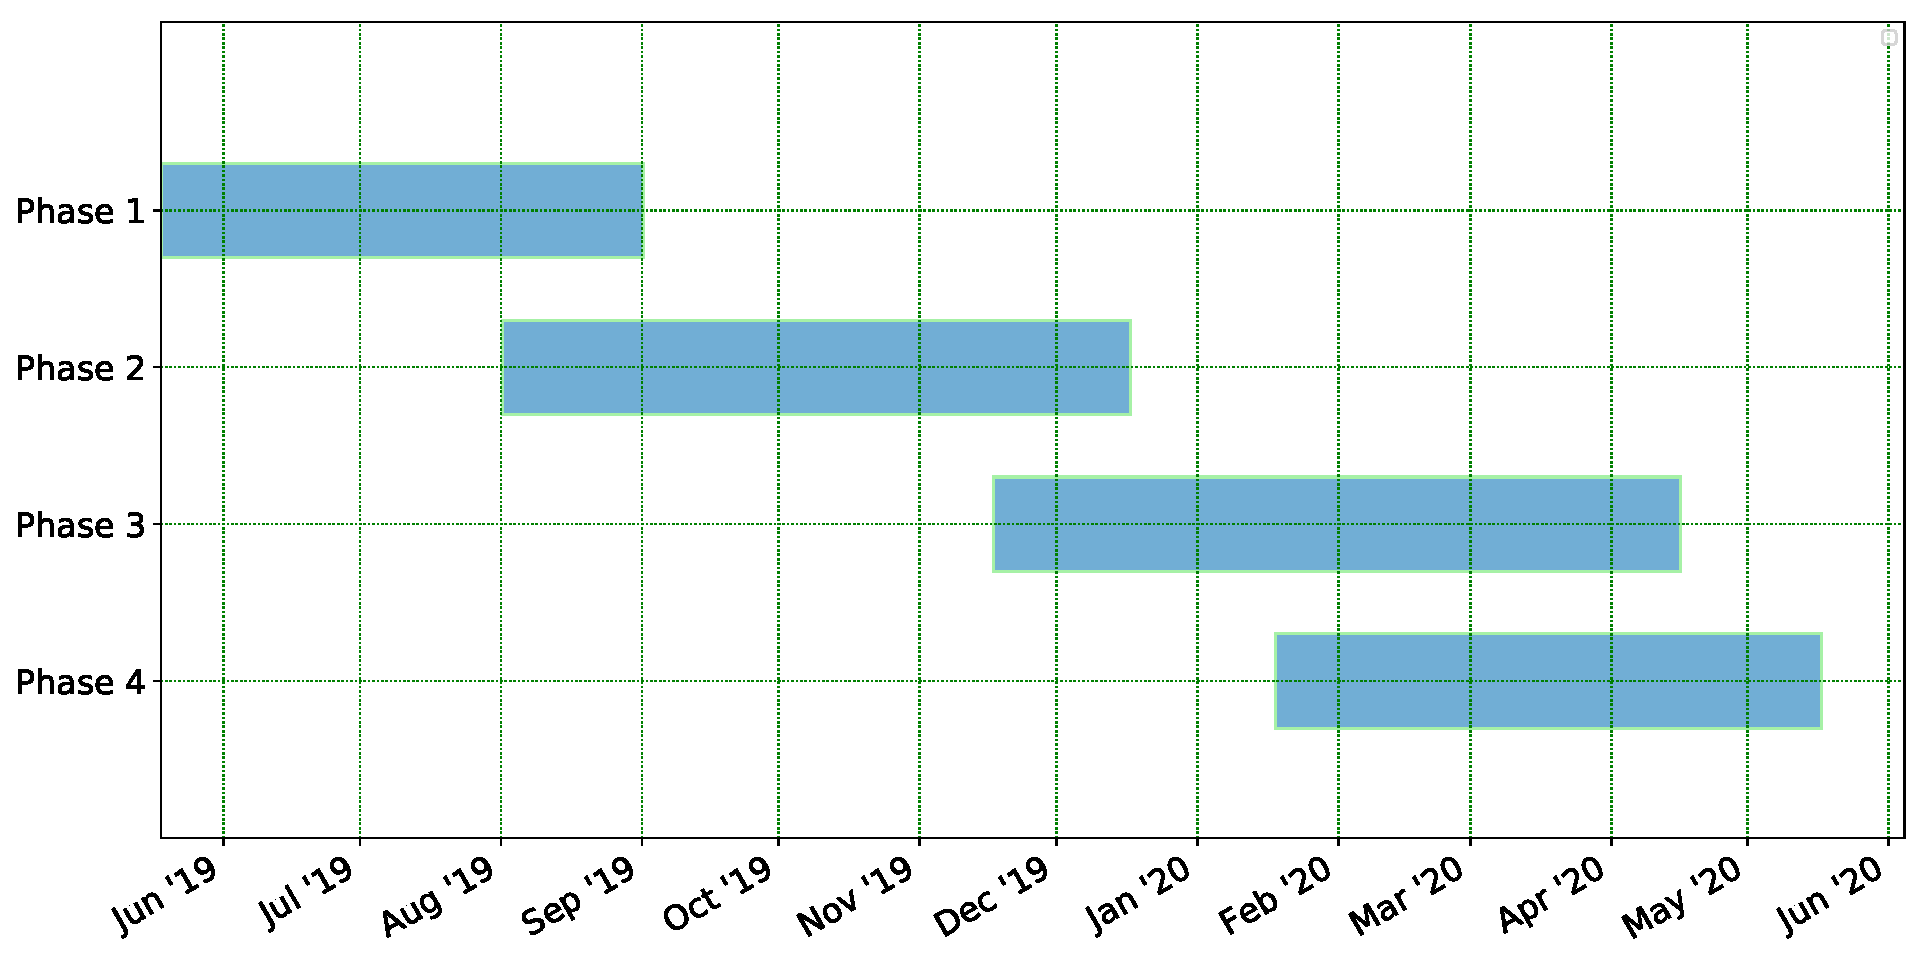
\includegraphics[width=.95\textwidth]{figures/phd_plan.pdf}
	\caption{Planned timeline of proposed research}\label{fig:work_plan}
\end{figure*}

\subsubsection{Phase 1: Design and implementation of a campaign manager}
Phase 1 would include design discussions for a prototype of the campaign manager.
Design a prototype is an iterative process, and it will provided the basic functionality of the campaign manager.
Result of these discussions will be the requirements of the campaign manager and its API. 
Design will be finalized and a prototypical implementation will be completed by Month 3. 
The prototype will interface with RADICAL-EnTK providing campaign execution capabilities.

\subsubsection{Phase 2: Implementation and performance analysis of makespan algorithm}
Phase 2 includes implementing the proposed algorithm in the prototype, supporting dynamic resources and understand its performance.
In case the selected algorithm under performs, a study will be conducted with additional makespan algorithms.
Phase 2 spans from months 3 up to 6.

\subsubsection{Phase 3: Experimental performance analysis}
Phase 3 of the plan includes an experimental performance analysis of the campaign manager for a set of selected use cases.
This performance analysis will compare the execution a computational campaign with the prototypical campaign manager and without.
This phase span between months 3 and 9.

% ---------------------------------------------------------------------------
% Why
\subsection{Significance and impact of work}
Several scientific campaigns require to execute a large number of workflows several times with different input data or initial conditions. 
The required concurrency to minimize the execution time of the campaign is not necessarily constant and may change based on resource availability. 
The campaign manager suggested in this proposal will be the first to make resource selection decisions for the users. 
This will lead to less time invested by users to make execution decisions about their workflows. 
These decisions will lead to better resource utilization and, as a result, better domain science. 
The empirical performance analysis derived by this work can be used to derive empirical models initial and eventually formal mathematical models.

% ---------------------------------------------------------------------------
% Challenges
\subsection{Challenges/Risks}

We estimate the proposed work, divided into three major phases, to take 9 months 
and we allocate 3 months to account for unforeseen circumstances. We would like 
to keep the committee aware of the following challenges that we see:

\begin{itemize}
	\item Design and Implementation (phase 1) is iterative and special attention needs to be given to the number of iterations against specific objectives, given the timeline.
    \item All experiments performed on HPC systems are subject to variable queue times and may limit the number of experiments performed in phase 2 and 3.
	\item Although the middleware will be well tested (80--90\% of the code base will be covered by unit tests) and less susceptible to major changes, RADICAL-Pilot is known to be less stable and is susceptible to changes as it serves multiple projects. Stability of RADICAL-Pilot is considered in the estimates, but needs to be made aware to the committee.
\end{itemize}

\bibliographystyle{plain}
\bibliography{proposal}
\end{document}